
\documentclass[xcolor={dvipsnames}]{beamer}
\usepackage{amsmath,amsfonts,amssymb,pxfonts,eulervm,xspace}
\usepackage{graphicx}
 \usepackage{multimedia}

\graphicspath{{./figures/}}
\usetheme{ccnycrest}


\newenvironment{changemargin}[2]{%
\begin{list}{}{%
\setlength{\topsep}{0pt}%
\setlength{\leftmargin}{#1}%
\setlength{\rightmargin}{#2}%
\setlength{\listparindent}{\parindent}%
\setlength{\itemindent}{\parindent}%
\setlength{\parsep}{\parskip}%
}%
\item[]}{\end{list}}

\begin{document}

\title{ CS102: Editor, Compiler and Hello World}
\author{Hannah Aizenman}


\begin{frame}
	\titlepage
\end{frame}

\begin{frame}[plain]	
	\begin{changemargin}{-1cm}{+0cm}
		\begin{figure}
			\includegraphics[width=1.20\textwidth]{subway}
		\end{figure}
	\end{changemargin}
\end{frame}

\begin{frame}[plain]	
	\begin{changemargin}{-1cm}{+0cm}
		\begin{figure}
			\includegraphics[width=1.20\textwidth]{subway_editor}
		\end{figure}
	\end{changemargin}
\end{frame}

\begin{frame}[plain]	
	\begin{changemargin}{-1cm}{+0cm}
		\begin{figure}
			\includegraphics[width=1.20\textwidth]{subway_editor_compiler}
		\end{figure}
	\end{changemargin}
\end{frame}

\begin{frame}{Editor: Plaintext}
	\begin{figure}
			\includegraphics[width=1\textwidth]{plaintext}
	\end{figure}
\end{frame}

\begin{frame}{Editor: Latex}
	\begin{figure}
			\includegraphics[width=1\textwidth]{slide}
	\end{figure}
\end{frame}

\begin{frame}{Editor: Code}
	\begin{figure}
			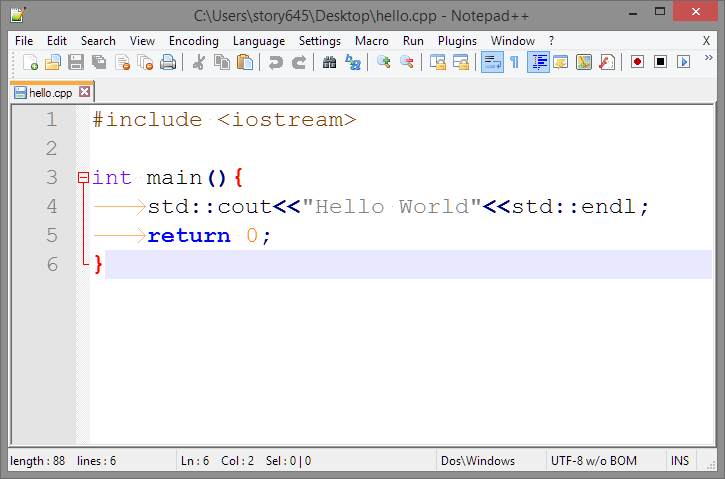
\includegraphics[width=1\textwidth]{code}
	\end{figure}
\end{frame}

\begin{frame}{Editor: Use}
	\begin{itemize}
	\item Use something simple that supports:
		\begin{itemize}
			\item code highlighting
			\item code folding
		\end{itemize}
	\pause
		\item Any platform:
		\begin{itemize} 
			\item terminal: vim, emacs, jed, nano
			\item graphical: sublime
		\end{itemize}
	\pause
		\item Windows: notepad++, notepad
		\item Mac: texwrangler, aquamacs, smultron
		\item Linux: kate, gedit, scite
	\end{itemize}
\end{frame}

\begin{frame}{Compiler}
		\href{http://krnlpanic.com/wp/c-compiler-basics/}{\includegraphics{compile1}}
		\pause
		\begin{block}{Stages}
		\begin{itemize}
			\item \textbf{Compiler:} Source code (.c/.cpp) converted into low level language (Assembly/.s)
			\pause
			\item \textbf{Assembler:} Assembly converted into machine code (object files/.o)
			\pause
			\item \textbf{Linker:} Links object files to prewritten/built-in functions and creates executable (.out/.exe)
		\end{itemize}
		\end{block}
\end{frame}

\begin{frame}{Compiler: Use}
	\begin{block}{Required for Class}
		\begin{center}
			gcc and  g++
		\end{center}
	\end{block}
	\pause
	\begin{block}{GNU Compiler Collection}
		\begin{itemize}
			\item GNU is a unix-like environment
			\item GNU components built into linux
			\item GNU emulators required for Windows/Mac
		\end{itemize}
	\end{block}
\end{frame}

\begin{frame}{GNU Emulators}
	\begin{itemize}
		\item Windows: MinGW or Cygwin
		\item Mac: homebrew 
			\begin{itemize}		
				\item xcode has to be installed for this to work\\
					but don't use xcode
			\end{itemize}
		\item Linux: don't need emulator, already baked in
		\item \textbf{Note}: Compiler run from terminal/command prompt
	\end{itemize}
\end{frame}

\begin{frame}{Hello World: Open Editor}
	\begin{figure}
			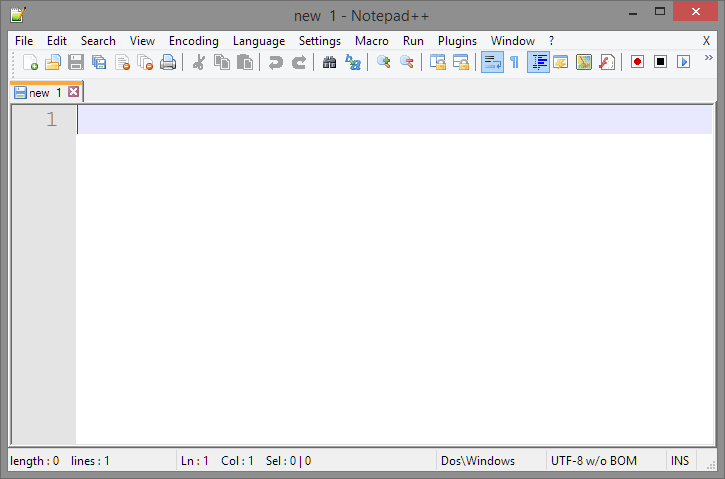
\includegraphics[width=1\textwidth]{empty}
	\end{figure}
\end{frame}

\begin{frame}{Hello World: Save as .cpp}
	\begin{figure}
			\includegraphics[width=1\textwidth]{initsave}
	\end{figure}
\end{frame}
\begin{frame}{Hello World: Include}
	\begin{figure}
			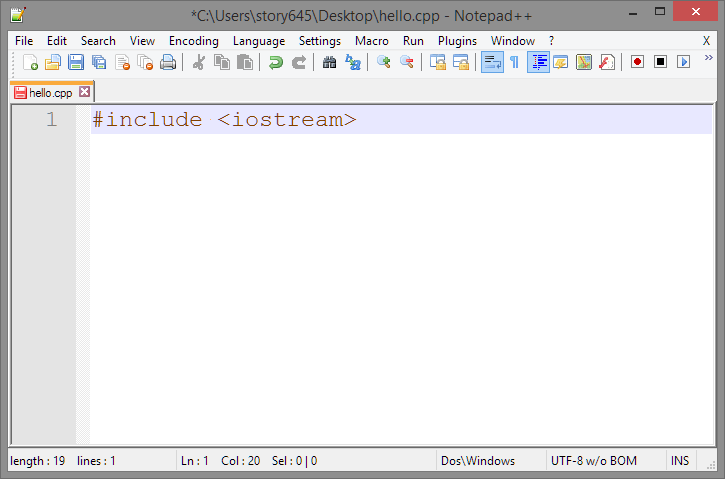
\includegraphics[width=1\textwidth]{include}
	\end{figure}
\end{frame}

\begin{frame}{Hello World: Namespace}
	\begin{figure}
			\includegraphics[width=1\textwidth]{namespace}
	\end{figure}
\end{frame}

\begin{frame}{Hello World: Main}
	\begin{figure}
			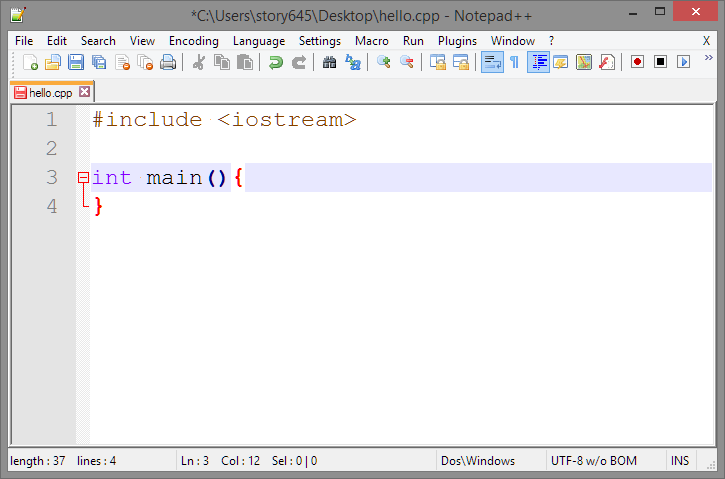
\includegraphics[width=1\textwidth]{main}
	\end{figure}
\end{frame}

\begin{frame}{Hello World: Cout}
	\begin{figure}
			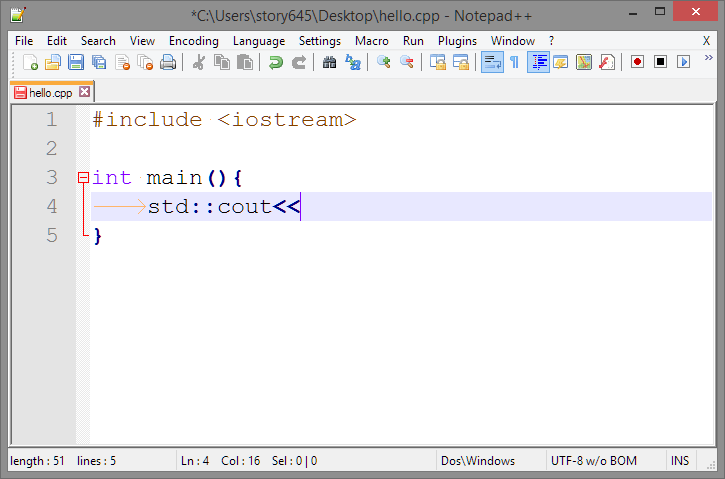
\includegraphics[width=1\textwidth]{cout}
	\end{figure}
\end{frame}

\begin{frame}{Hello World: Hello}
	\begin{figure}
			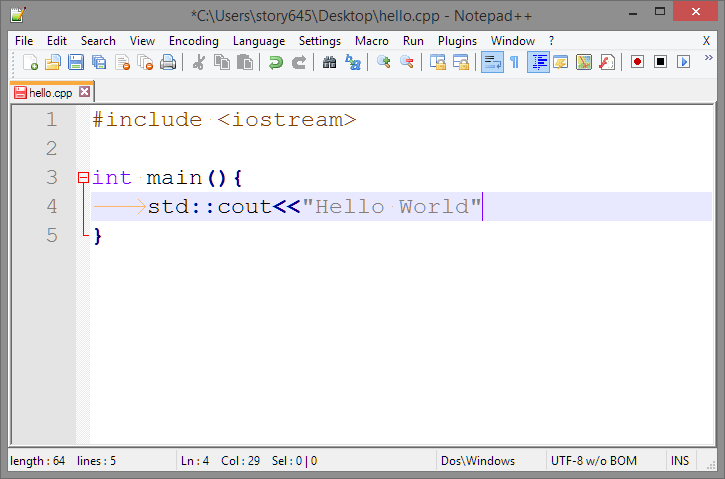
\includegraphics[width=1\textwidth]{hello}
	\end{figure}
\end{frame}

\begin{frame}{Hello World: Endl}
	\begin{figure}
			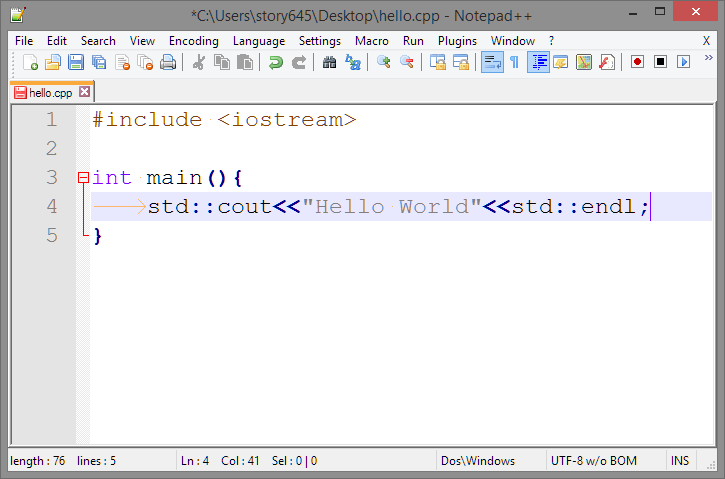
\includegraphics[width=1\textwidth]{endl}
	\end{figure}
\end{frame}

\begin{frame}{Hello World: Return}
	\begin{figure}
			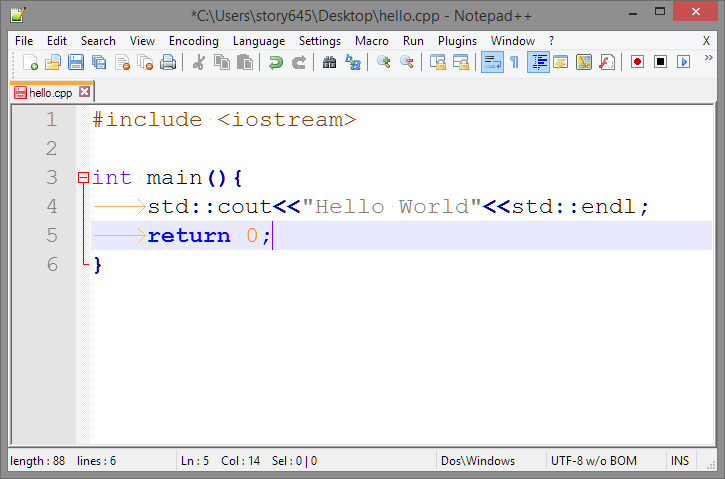
\includegraphics[width=1\textwidth]{return}
	\end{figure}
\end{frame}

\begin{frame}{Hello World: Save}
	\begin{figure}
			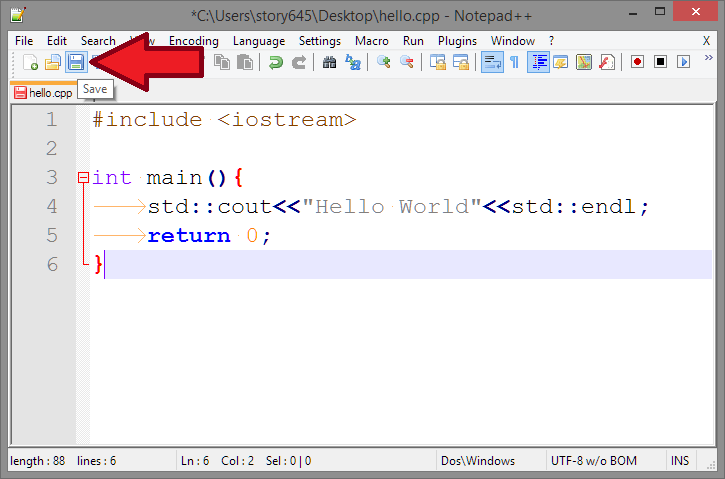
\includegraphics[width=1\textwidth]{save}
	\end{figure}
\end{frame}

\begin{frame}{Hello World: Saved}
	\begin{figure}
			\includegraphics[width=1\textwidth]{Saved}
	\end{figure}
\end{frame}

\begin{frame}{Hello World: cd}
	\begin{figure}
			\includegraphics[width=1\textwidth]{cd}
	\end{figure}
\end{frame}

\begin{frame}{Hello World: Compile}
	\begin{figure}
			\includegraphics[width=1\textwidth]{compile}
	\end{figure}
\end{frame}

\begin{frame}{Hello World: Compiled}
	\begin{figure}
			\includegraphics[width=1\textwidth]{compiled}
	\end{figure}
\end{frame}

\begin{frame}{Hello World: Execute}
	\begin{figure}
			\includegraphics[width=1\textwidth]{execute}
	\end{figure}
\end{frame}

\begin{frame}{Hello World: Execute}
	\begin{figure}
			\includegraphics[width=1\textwidth]{executed}
	\end{figure}
\end{frame}

\end{document}

